\chapter{La différenciation cellulaire~: la cellule musculaire squelettique}\label{ch:b2:cell-differentiation}

Une fibre de votre muscle de la cuisse est une cellule unique longue de
trente centimètres, pourvue de centaines de noyaux, remplie d'un bout à
l'autre de bâtonnets contractiles si réguliers qu'elle paraît striée au
microscope. Elle a commencé sous la forme d'un amas de cellules d'aspect
ordinaire qui ont quitté un somite en rampant, se sont multipliées, ont
cessé de se diviser, se sont alignées, ont fusionné et ont activé
plusieurs centaines de gènes qu'elles n'avaient jamais utilisés. Toutes
les cellules du corps possèdent le même génome~; une \omterm{def:b2:cell-differentiation:myogenesis}{fibre musculaire}
est ce que fait ce génome lorsqu'un \omterm{prop:b2:cell-differentiation:transcriptional}{facteur de transcription} particulier
est activé. Ce chapitre prend la cellule musculaire squelettique comme
exemple détaillé de \emph{\omterm{def:b2:cell-differentiation:differentiation}{différenciation}} --- la manière dont une
cellule acquiert et conserve une identité spécialisée --- et la cellule
musculaire est un bon exemple, car l'interrupteur principal est connu,
les étapes peuvent être observées dans une boîte de culture, et la
cellule achevée est une machine dont les pièces sont visibles.

\section{Ce qu'est la différenciation}

\begin{definition}[Différenciation, détermination, potentialité]\label{def:b2:cell-differentiation:differentiation}
\index{differenciation@différenciation}\index{determination@détermination}\index{cellule souche}\index{potentialite@potentialité}
Une cellule est \emph{différenciée} lorsqu'elle exprime le profil stable
de gènes --- et donc les protéines, la forme et la fonction --- d'un type
cellulaire. Elle est \emph{déterminée} (ou engagée) lorsque son destin
est fixé bien que sa différenciation n'ait pas encore commencé~: un
\omterm{def:b2:cell-differentiation:myogenesis}{myoblaste} ressemble à un fibroblaste mais ne formera que du muscle. La
\emph{potentialité} est l'éventail des types qu'une cellule peut encore
produire~: \emph{totipotente} (le zygote et les premiers blastomères,
qui forment tout, y compris le \omterm{def:b2:mammal-reproduction:placenta}{placenta}), \emph{pluripotente} (la \omterm{def:b2:mammal-reproduction:implantation}{masse
cellulaire interne}, qui forme tous les tissus du corps),
\emph{multipotente} (une cellule souche du sang ou du muscle, qui forme
les types d'un tissu), \emph{unipotente}. Une \emph{cellule souche} est
une cellule qui se divise en donnant une cellule fille semblable à
elle-même et une autre qui poursuit sa différenciation, ce qui maintient
le stock tout en approvisionnant le tissu. La différenciation n'est,
dans la plupart des cas, pas une perte de gènes mais un choix parmi eux~:
le génome d'un noyau musculaire est complet.
\end{definition}
\begin{proof}[Faits expérimentaux]
Gurdon (1962) transplanta le noyau d'une cellule intestinale
différenciée de têtard dans un œuf de grenouille dont le noyau avait
été détruit~; une partie des œufs se développèrent en grenouilles
normales et fertiles. Le noyau différencié n'avait perdu aucun des
gènes nécessaires pour construire un animal entier~; le cytoplasme de
l'œuf l'avait réinitialisé. La même opération avec un noyau de cellule
mammaire dans un ovocyte de brebis donna Dolly (1996), et la
reprogrammation d'un fibroblaste de peau en \omterm{def:b2:cell-differentiation:differentiation}{cellule souche} pluripotente
par quatre \omterm{prop:b2:cell-differentiation:transcriptional}{facteurs de transcription} (Yamanaka, 2006) montra que cette
réinitialisation peut se faire avec une poignée de protéines.
\end{proof}

\begin{proposition}[La différenciation est transcriptionnelle]\label{prop:b2:cell-differentiation:transcriptional}
\index{facteur de transcription}\index{regulateur maitre@régulateur maître}
La différence entre deux types cellulaires tient aux gènes qui sont
transcrits. Quelques \emph{\omterm{prop:b2:cell-differentiation:transcriptional}{facteurs de transcription}}, exprimés en
réponse aux signaux inducteurs du
\cref{ch:b2:vertebrate-development}, se fixent sur les régions
régulatrices de centaines de gènes cibles et les activent, tandis que
les gènes des autres destins sont éteints~; et comme un tel facteur
active souvent son propre gène, l'état, une fois atteint, s'entretient
de lui-même. Pour certains tissus, un seul facteur est un
\emph{\omterm{prop:b2:cell-differentiation:transcriptional}{régulateur maître}} suffisant pour imposer le destin à une cellule
d'un autre type~: \omterm{def:b2:cell-differentiation:myogenesis}{MyoD} pour le muscle squelettique, Pax6 pour l'œil,
Sox9 pour le cartilage. L'état est encore stabilisé par des
modifications de la chromatine --- méthylation de l'ADN, modification
des histones --- qui maintiennent silencieux les gènes éteints au fil
des divisions (l'\emph{épigénétique} du volume de troisième année). Une
cellule différenciée se souvient donc de ce qu'elle est sans aucune
modification de sa séquence d'ADN, et cette mémoire est inscrite dans
le profil des facteurs et de la chromatine, non dans les gènes.
\end{proposition}

\section{La construction d'une fibre musculaire}

\begin{definition}[La myogenèse]\label{def:b2:cell-differentiation:myogenesis}
\index{myoblaste}\index{myotube}\index{fibre musculaire}\index{MyoD}
Chez l'embryon, des cellules du dermomyotome du somite sont induites,
par des signaux issus du \omterm{prop:b2:vertebrate-development:neurulation}{tube neural}, de la notocorde et de l'ectoderme
de surface, à exprimer les facteurs myogéniques \emph{MyoD} et
\emph{Myf5}~: ce sont désormais des \emph{myoblastes}, déterminés mais
encore en division et d'aspect banal. Les myoblastes migrent --- dans
les \omterm{def:b2:limb-organogenesis:bud}{bourgeons de membres}, par exemple --- et se multiplient tant que des
facteurs de croissance (FGF) sont présents. Lorsque ces facteurs
s'épuisent, ils sortent du cycle cellulaire, expriment un second
facteur, la \emph{myogénine}, s'alignent bout à bout et
\emph{fusionnent}~: leurs membranes se confondent en un \emph{myotube}
unique et allongé, aux nombreux noyaux alignés. Le myotube active les
gènes musculaires --- actine, myosine, troponine, tropomyosine, créatine
kinase, récepteur de l'acétylcholine --- assemble l'appareil contractile
et mûrit en une \emph{fibre musculaire} dont les noyaux se trouvent à la
périphérie. Une fibre ne se divise plus jamais~; quelques myoblastes
restent à côté d'elle, quiescents, sous forme de \emph{cellules
satellites}, les \omterm{def:b2:cell-differentiation:differentiation}{cellules souches} qui réparent et font croître le
muscle toute la vie durant.
\end{definition}

\begin{omfigure}
\begin{tikzpicture}[every node/.style={font=\scriptsize}, >=stealth]
  % somite
  \draw[thick, fill=omProp!25] (0,0) ellipse (0.6 and 0.5); \node[below, align=center] at (0,-0.6) {somite\\(dermomyotome)};
  \draw[->, thick] (0.7,0) -- (1.6,0) node[midway, above=0.35cm, align=center] {induction\\Wnt, Shh};
  % myoblasts dividing
  \foreach \p in {(2.2,0.3),(2.7,-0.3),(3.2,0.3),(3.7,-0.3)} \draw[thick, fill=omDef!25] \p ellipse (0.28 and 0.18);
  \node[below, align=center] at (3.0,-0.6) {myoblastes~: MyoD, Myf5\\division en présence de FGF};
  \draw[->, thick] (4.1,0) -- (5.0,0) node[midway, above=0.45cm, align=center] {retrait du FGF~:\\myogénine,\\sortie du cycle};
  % aligned, fusing
  \foreach \x in {5.35,5.95,6.55,7.15} \draw[thick, fill=omDef!25] (\x,0) ellipse (0.3 and 0.16);
  \node[below, align=center] at (6.25,-0.6) {alignement et fusion};
  \draw[->, thick] (7.6,0) -- (8.5,0);
  % myotube
  \draw[thick, fill=omDef!15, rounded corners=6pt] (8.7,-0.3) rectangle (12.6,0.3);
  \foreach \x in {9.2,10.0,10.8,11.6,12.3} \fill[omDef!80!black] (\x,0) ellipse (0.13 and 0.08);
  \node[below, align=center] at (10.65,-0.6) {myotube~: nombreux noyaux,\\gènes musculaires activés, myofibrilles assemblées};
\end{tikzpicture}

{\small La myogenèse~: des cellules du somite induites deviennent des
\omterm{def:b2:cell-differentiation:myogenesis}{myoblastes} qui se divisent~; lorsque les facteurs de croissance sont
retirés, ils cessent de se diviser, s'alignent et fusionnent en un
\omterm{def:b2:cell-differentiation:myogenesis}{myotube} plurinucléé qui active les gènes musculaires.}
\end{omfigure}

\begin{omfigure}
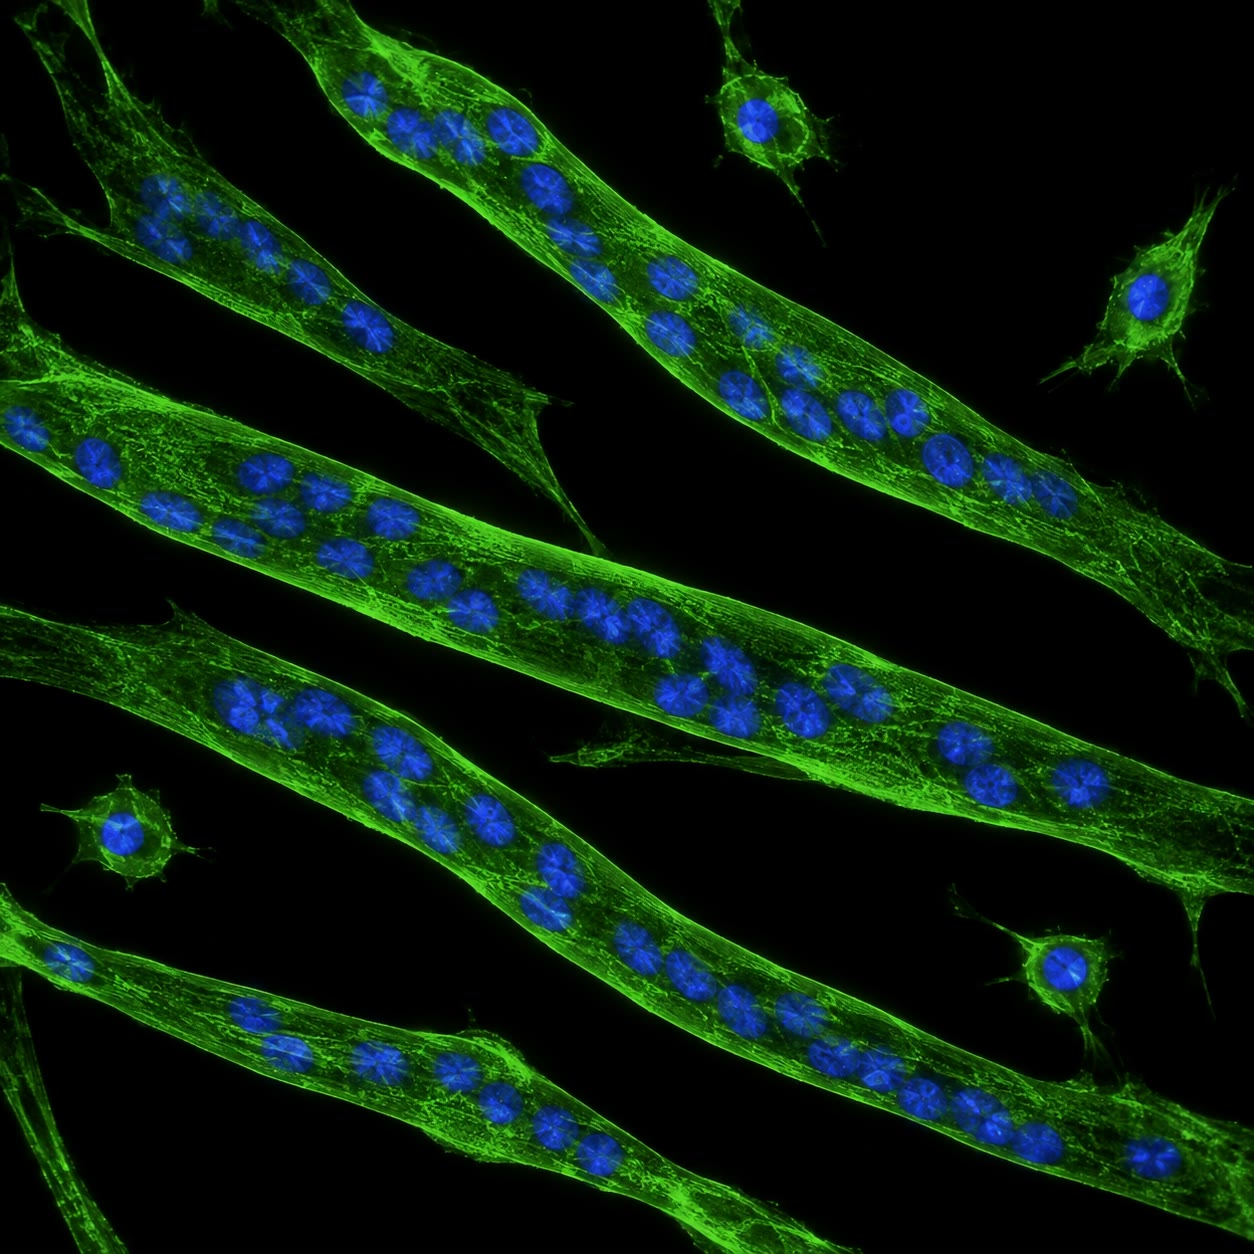
\includegraphics[width=0.44\linewidth]{images/book4/ai/b4-12-myotubes.jpg}\hspace{0.04\linewidth}
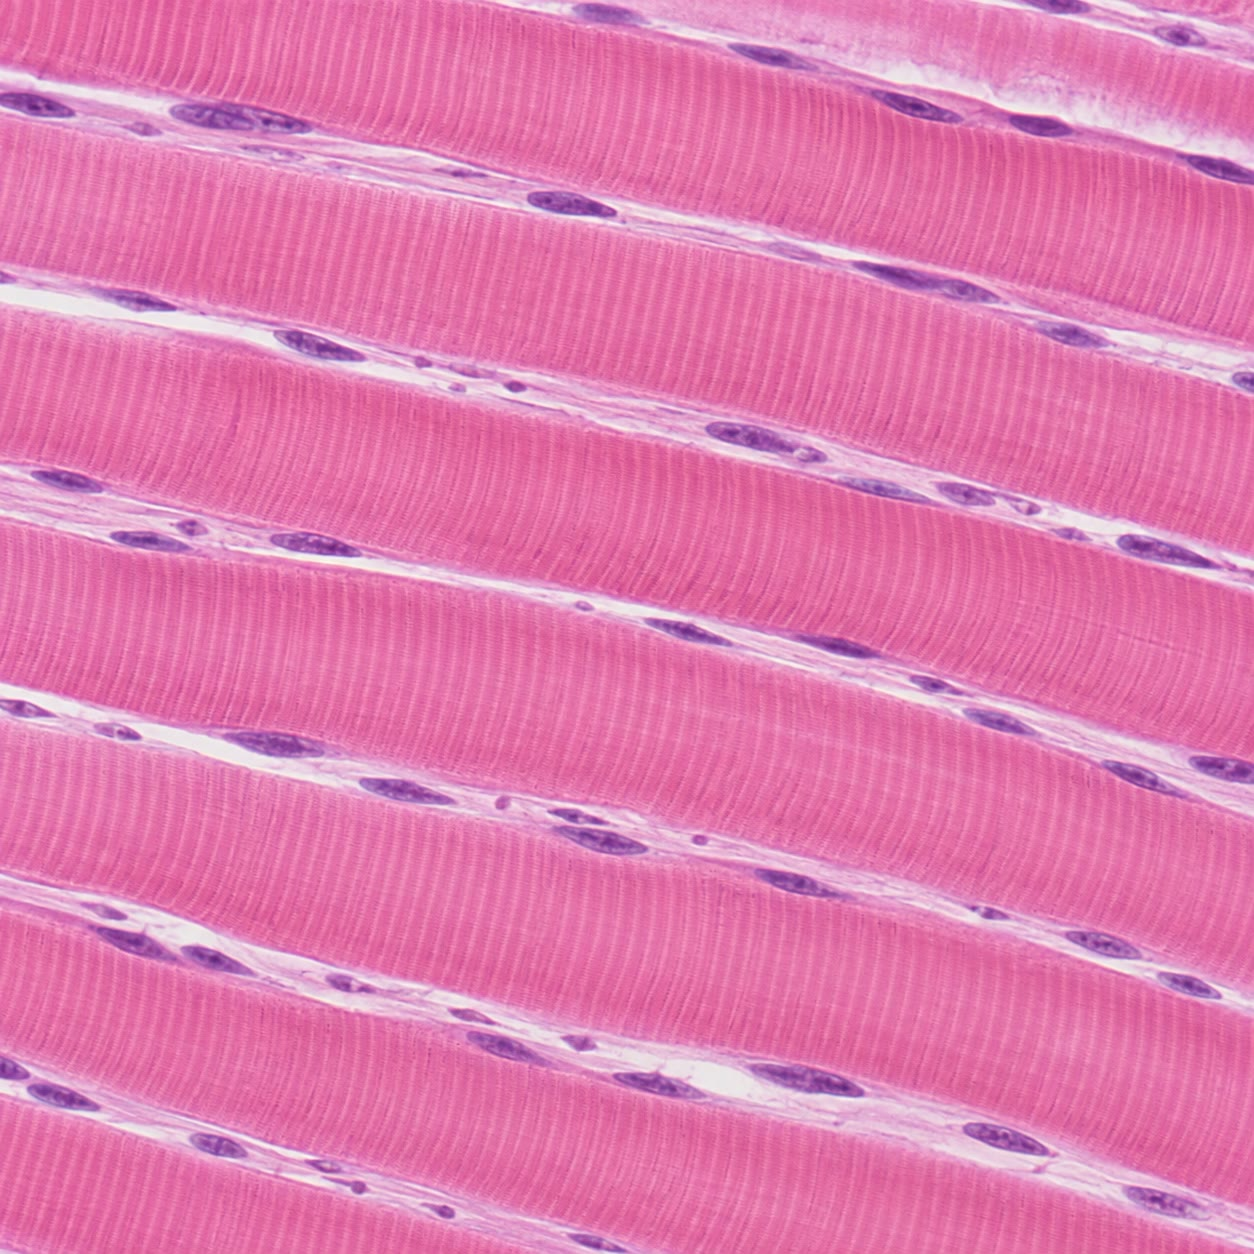
\includegraphics[width=0.44\linewidth]{images/book4/ai/b4-12-muscle-fibres.jpg}

{\small À gauche~: des \omterm{def:b2:cell-differentiation:myogenesis}{myotubes} en culture, chacun une cellule fusionnée
portant une rangée de noyaux, à côté de \omterm{def:b2:cell-differentiation:myogenesis}{myoblastes} isolés qui n'ont pas
encore fusionné. À droite~: des fibres mûres vues en long, leurs
striations transversales correspondant aux \omterm{def:b2:cell-differentiation:fibre}{sarcomères} répétés et leurs
noyaux repoussés à la périphérie.}
\end{omfigure}

\begin{proposition}[MyoD~: un interrupteur principal]\label{prop:b2:cell-differentiation:myod}
\index{regulateur maitre!MyoD@régulateur maître!MyoD}
\omterm{def:b2:cell-differentiation:myogenesis}{MyoD} est un \omterm{prop:b2:cell-differentiation:transcriptional}{facteur de transcription} de la famille hélice-boucle-hélice.
Il se fixe, sous forme de dimère avec une protéine partenaire ubiquitaire,
sur une séquence de six bases (la boîte E, CANNTG) des régions
régulatrices des gènes musculaires, recrute des enzymes qui ouvrent la
chromatine et active les gènes --- y compris les gènes de la myogénine et
de \omterm{def:b2:cell-differentiation:myogenesis}{MyoD} lui-même, ce qui maintient l'état. Son activité est contrôlée~:
dans les \omterm{def:b2:cell-differentiation:myogenesis}{myoblastes} en division, une protéine inhibitrice (Id), induite
par les facteurs de croissance, séquestre le partenaire et maintient
\omterm{def:b2:cell-differentiation:myogenesis}{MyoD} inactif~; lorsque les facteurs de croissance sont retirés, Id
disparaît et \omterm{def:b2:cell-differentiation:myogenesis}{MyoD} agit. Comme \omterm{def:b2:cell-differentiation:myogenesis}{MyoD} suffit à imposer le programme
musculaire à un fibroblaste, à une cellule adipeuse ou à une cellule
nerveuse, le destin musculaire ne tient, en un sens, qu'à un seul gène~:
la difficulté de devenir un muscle n'est pas de savoir comment faire,
mais de recevoir l'ordre de le faire.
\end{proposition}
\begin{proof}[Faits expérimentaux]
Davis, Weintraub et Lassar (1987) transférèrent un seul ADNc, isolé à
partir de \omterm{def:b2:cell-differentiation:myogenesis}{myoblastes}, dans des fibroblastes en culture~: les fibroblastes
cessèrent de se diviser, fusionnèrent en \omterm{def:b2:cell-differentiation:myogenesis}{myotubes} et fabriquèrent des
protéines musculaires. Le gène fut nommé \omterm{def:b2:cell-differentiation:myogenesis}{MyoD}. Ses apparentés Myf5,
myogénine et MRF4 furent trouvés par homologie~; une souris dépourvue à
la fois de \omterm{def:b2:cell-differentiation:myogenesis}{MyoD} et de Myf5 n'a ni \omterm{def:b2:cell-differentiation:myogenesis}{myoblastes} ni muscle squelettique,
tandis qu'une souris dépourvue de myogénine a des \omterm{def:b2:cell-differentiation:myogenesis}{myoblastes} qui ne
fusionnent jamais.
\end{proof}

\begin{theorem}[Un interrupteur qui s'entretient lui-même]\label{thm:b2:cell-differentiation:switch}
\index{bistabilite@bistabilité}\index{retroaction positive!gene@rétroaction positive!gène}
Soit $m$ la quantité d'un facteur qui active son propre gène avec une
réponse coopérative (sigmoïde) et qui est dégradé avec une constante $k$~:
\[
\frac{\mathrm{d}m}{\mathrm{d}t} = \frac{a\,m^{2}}{K^{2} + m^{2}} + b - k\,m,
\]
où $b$ est une faible synthèse basale. Pour des valeurs convenables de
$a$, $b$, $K$ et
$k$, cette équation possède \emph{deux} états stationnaires stables, un
état bas voisin de $b/k$ et un état haut voisin de $a/k$, séparés par un
seuil instable~: la cellule est \emph{bistable}. Un signal inducteur
transitoire qui fait passer $m$ au-dessus du seuil envoie la cellule
dans l'état haut, où elle reste après la disparition du signal~; en
dessous du seuil, elle retourne à l'état bas. C'est une mémoire
construite à partir d'une boucle de rétroaction, et c'est pourquoi une
cellule, une fois engagée, reste engagée au fil des divisions et en
l'absence de l'inducteur.
\end{theorem}
\begin{proof}
Les états stationnaires vérifient $k m = a m^{2}/(K^{2} + m^{2}) + b$. Le
membre de droite est une sigmoïde qui monte de $b$ à $a + b$~; celui de
gauche est une droite passant par l'origine, de pente $k$. Pour
$b/k < K$ et $k$ assez petit pour que la droite coupe la partie raide
de la sigmoïde, les deux courbes se coupent trois fois~: en
$m_{\text{bas}} \approx b/k$, en une valeur intermédiaire
$m_{\text{i}}$, et en $m_{\text{haut}} \approx (a +
b)/k$. Stabilité~: en dessous de $m_{\text{bas}}$, la synthèse dépasse
la dégradation et $m$ augmente~; entre $m_{\text{bas}}$ et
$m_{\text{i}}$, la dégradation dépasse la synthèse et $m$ redescend~;
entre $m_{\text{i}}$ et
$m_{\text{haut}}$, la synthèse dépasse la dégradation et $m$ monte
jusqu'à $m_{\text{haut}}$~; au-dessus, $m$ redescend vers
$m_{\text{haut}}$. Les deux états extrêmes sont donc stables, celui du
milieu est instable et constitue le seuil.
\end{proof}

\begin{omfigure}
\begin{tikzpicture}
\begin{axis}[
  width=0.74\linewidth, height=5.8cm,
  axis x line=bottom, axis y line=left,
  xmin=0, xmax=4, ymin=0, ymax=1.3,
  xlabel={niveau du facteur $m$ (relatif)}, ylabel={vitesse},
  xlabel style={font=\small, at={(axis description cs:0.5,-0.12)}, anchor=north},
  ylabel style={font=\small},
  tick label style={font=\small}, xtick={0,1,2,3,4}, ytick={0,0.5,1},
  legend style={font=\scriptsize, at={(0.03,0.97)}, anchor=north west, draw=none},
  clip=false,
]
\addplot[very thick, omDef, domain=0:4, samples=100] {x^2/(1+x^2) + 0.02};
\addlegendentry{synthèse~: $a m^2/(K^2 + m^2) + b$}
\addplot[very thick, omThm, domain=0:3.2, samples=2] {0.4*x};
\addlegendentry{dégradation~: $k m$}
\fill[omDef] (axis cs:0.055,0.022) circle (2pt); \draw[gray] (axis cs:0.08,0.04) -- (axis cs:0.33,0.42); \node[font=\scriptsize, anchor=west] at (axis cs:0.35,0.45) {éteint};
\draw[gray, thick] (axis cs:0.41,0.164) circle (2pt); \node[font=\scriptsize, anchor=west] at (axis cs:0.55,0.10) {seuil};
\fill[omDef] (axis cs:2.1,0.84) circle (2pt); \node[font=\scriptsize, anchor=north] at (axis cs:2.1,0.78) {allumé};
\end{axis}
\end{tikzpicture}

{\small Un interrupteur bistable ($a = 1$, $K = 1$, $b = 0.02$, $k = 0.4$).
La synthèse (sigmoïde) et la dégradation (droite) se coupent trois
fois~: deux états stables, éteint et allumé, et un seuil instable entre
les deux. Un signal qui fait franchir le seuil à $m$ engage
définitivement la cellule dans l'état allumé.}
\end{omfigure}

\section{La cellule achevée}

\begin{definition}[La fibre musculaire]\label{def:b2:cell-differentiation:fibre}
\index{sarcomere@sarcomère}\index{myofibrille}\index{reticulum sarcoplasmique@réticulum sarcoplasmique}\index{tubule T}
Une \omterm{def:b2:cell-differentiation:myogenesis}{fibre musculaire} squelettique est un cylindre de
\qtyrange{10}{100}{\micro m} de diamètre et long de plusieurs dizaines
de centimètres au plus, limité par le \emph{sarcolemme}, sous lequel se
trouvent des centaines de noyaux. Son intérieur est rempli de
\emph{myofibrilles} parallèles, chacune étant une chaîne de
\emph{sarcomères} longs de \qty{2.5}{\micro m}~: entre deux stries Z,
des filaments fins d'actine (avec la tropomyosine et la troponine),
ancrés aux stries Z, s'intercalent entre des filaments épais de myosine
maintenus au centre, et ce motif de chevauchement donne les striations.
Autour de chaque myofibrille, une dentelle de \emph{réticulum
sarcoplasmique} stocke le calcium~; les \emph{tubules transverses},
invaginations du sarcolemme, courent entre les myofibrilles et
transmettent le signal électrique de la surface vers l'intérieur. Des
mitochondries occupent les espaces, et le cytoplasme contient du
glycogène, de la créatine phosphate et, dans les fibres rouges, de la
myoglobine. La cellule est construite pour une seule chose --- se
raccourcir sur commande --- et le mécanisme de cette commande fait
l'objet du
\cref{ch:b2:muscle-movement}.
\end{definition}

\begin{omfigure}
\begin{tikzpicture}[every node/.style={font=\scriptsize}]
  % a stretch of myofibril with two sarcomeres
  \foreach \s in {0,4.4} {
    \begin{scope}[xshift=\s cm]
      \draw[very thick, omThm] (0,-1.1) -- (0,1.1);
      \foreach \y in {-0.9,-0.5,-0.1,0.3,0.7} { \draw[thick, omDef] (0,\y) -- (1.6,\y); \draw[thick, omDef] (4.4,\y) -- (2.8,\y); }
      \foreach \y in {-0.7,-0.3,0.1,0.5,0.9} { \draw[line width=3pt, omExo!80!black] (1.0,\y) -- (3.4,\y); }
      \draw[gray] (2.2,-1.1) -- (2.2,1.1);
    \end{scope}
  }
  \draw[very thick, omThm] (8.8,-1.1) -- (8.8,1.1);
  \node[omThm, below] at (0,-1.15) {strie Z};
  \node[omThm, below] at (4.4,-1.15) {strie Z};
  \node[omThm, below] at (8.8,-1.15) {strie Z};
  \node[omDef, above] at (0.8,1.15) {filaments fins (actine)};
  \node[omExo!80!black, above] at (6.6,1.15) {filaments épais (myosine)};
  \node[gray, below] at (2.2,-1.15) {ligne M};
  \draw[<->] (0,1.9) -- (4.4,1.9); \node[above] at (2.2,1.9) {un sarcomère, \qty{2.5}{\micro m}};
  \draw[<->] (5.4,-1.6) -- (7.8,-1.6); \node[below] at (6.6,-1.6) {bande A (sombre)};
  \draw[<->] (7.8,-1.6) -- (9.8,-1.6); \node[below] at (8.8,-1.6) {bande I (claire)};
\end{tikzpicture}

{\small Deux \omterm{def:b2:cell-differentiation:fibre}{sarcomères} d'une \omterm{def:b2:cell-differentiation:fibre}{myofibrille}~: les filaments fins d'actine,
ancrés aux stries Z, s'intercalent entre les filaments épais de myosine
centrés sur la ligne M. Le chevauchement donne la bande A sombre et la
bande I claire des striations.}
\end{omfigure}

\begin{proposition}[Les types de fibres]\label{prop:b2:cell-differentiation:types}
\index{types de fibres musculaires}
Un muscle est un mélange de types de fibres, déterminés en partie par la
lignée des \omterm{def:b2:cell-differentiation:myogenesis}{myoblastes} et en partie par le nerf qui innerve la fibre. Les
fibres \emph{lentes oxydatives} (type I) possèdent une myosine lente, de
nombreuses mitochondries et de nombreux capillaires, et de la myoglobine
--- rouges, infatigables, faites pour la posture et l'endurance. Les
fibres \emph{rapides glycolytiques} (type IIx) possèdent une myosine
rapide, peu de mitochondries et beaucoup de glycogène --- blanches,
puissantes, épuisées en une minute. Les fibres \emph{rapides oxydatives}
(type IIa) sont intermédiaires. Le mollet d'un sprinteur est surtout
fait de fibres rapides, celui d'un marathonien surtout de fibres lentes,
et ces proportions sont héréditaires~; mais le type n'est pas figé~:
l'innervation croisée d'un muscle rapide par un nerf lent, ou des mois
d'entraînement en endurance, convertissent des fibres vers le type lent,
car le profil des influx nerveux commute les gènes des isoformes de la
myosine et ceux de la biogenèse mitochondriale. Une cellule différenciée
garde son identité de \omterm{def:b2:cell-differentiation:myogenesis}{fibre musculaire} tout en révisant son programme
en fonction de l'usage.
\end{proposition}

\begin{example}[Croissance et réparation]\label{ex:b2:cell-differentiation:satellite}
Chez l'adulte, un muscle croît non pas en ajoutant des fibres mais en
les agrandissant~: l'entraînement ajoute des \omterm{def:b2:cell-differentiation:fibre}{myofibrilles} à chaque
fibre, et des \emph{cellules satellites} fusionnent avec elle pour
fournir les noyaux supplémentaires dont a besoin un cytoplasme plus
volumineux. Après une lésion, les mêmes cellules se divisent,
réexpriment \omterm{def:b2:cell-differentiation:myogenesis}{MyoD}, fusionnent et reconstruisent le segment endommagé en
quelques semaines --- le programme embryonnaire exécuté de nouveau chez
l'adulte. Dans la myopathie, les fibres sont dépourvues de dystrophine,
une protéine qui relie les \omterm{def:b2:cell-differentiation:fibre}{myofibrilles} à la membrane, et se déchirent
pendant la contraction~; les cellules satellites les réparent encore et
encore jusqu'à ce que, au bout d'années, le stock soit épuisé et que du
tissu fibreux prenne la place du muscle.
\end{example}

\begin{omfigure}
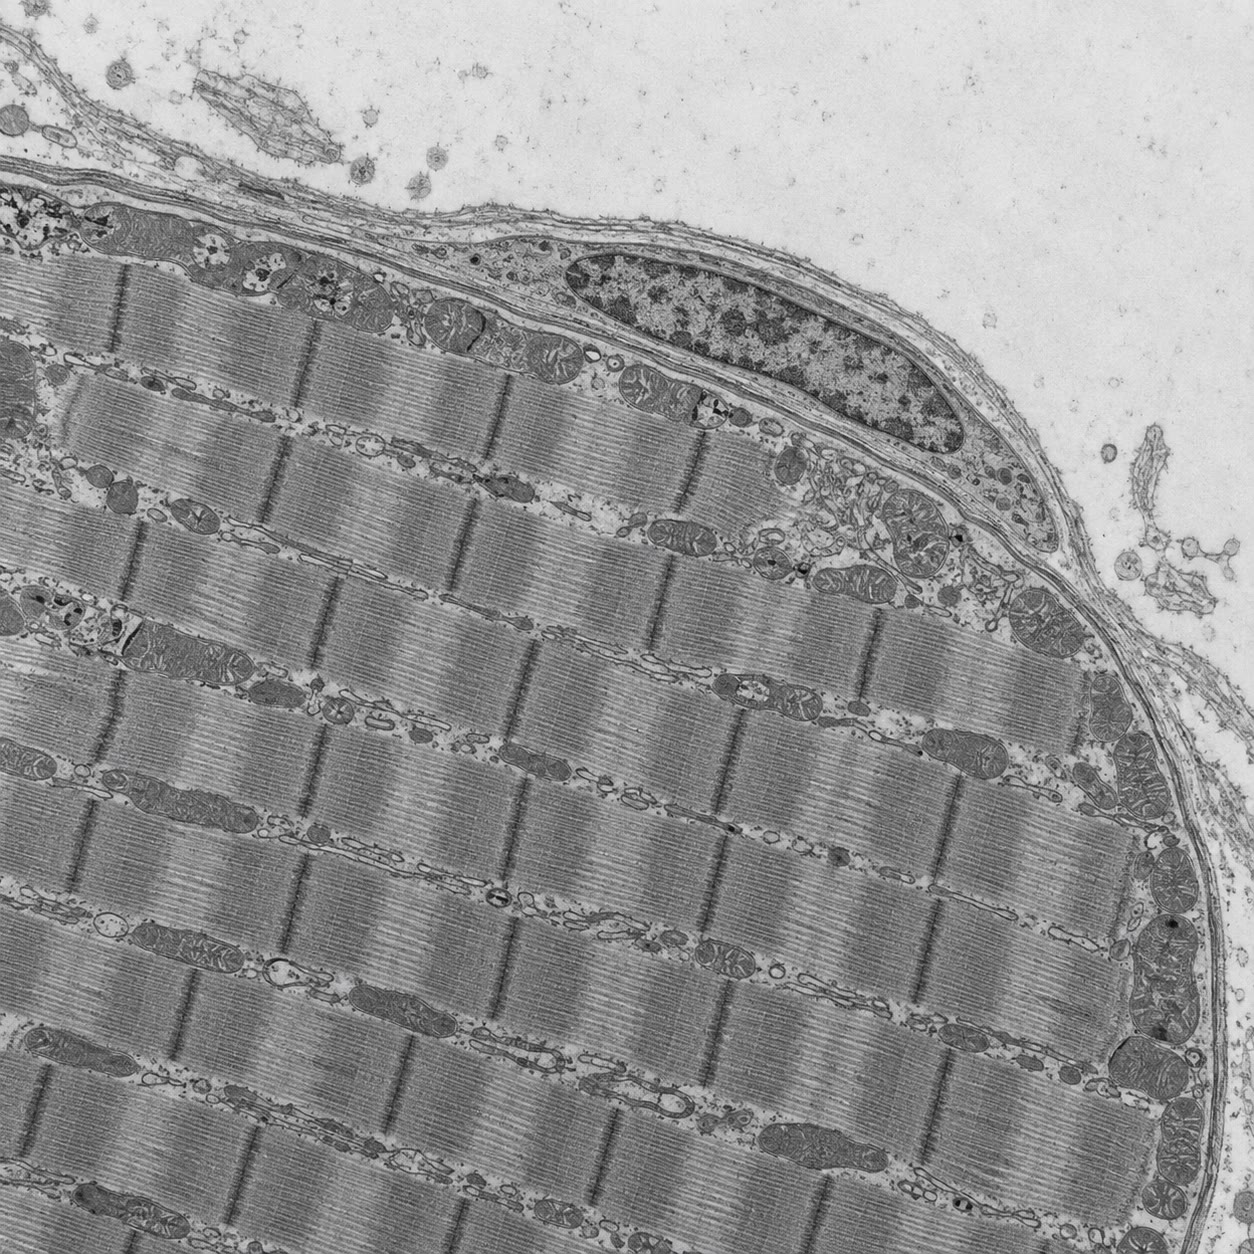
\includegraphics[width=0.42\linewidth]{images/book4/ai/b4-12-satellite-cell-tem.jpg}

{\small Une cellule satellite au microscope électronique~: une petite
cellule mononucléée logée entre la membrane d'une \omterm{def:b2:cell-differentiation:myogenesis}{fibre musculaire} et sa
lame basale --- la réserve de \omterm{def:b2:cell-differentiation:myogenesis}{myoblastes} de la fibre.}
\end{omfigure}

\section{Exercices}

\begin{exercise}[$\star$]\label{exo:b2:cell-differentiation:1}
Définir \omterm{def:b2:cell-differentiation:differentiation}{différenciation}, \omterm{def:b2:cell-differentiation:differentiation}{détermination} et \omterm{def:b2:cell-differentiation:differentiation}{potentialité}, et placer le
zygote, une cellule de la \omterm{def:b2:mammal-reproduction:implantation}{masse cellulaire interne}, une cellule
satellite et une \omterm{def:b2:cell-differentiation:myogenesis}{fibre musculaire} sur l'échelle des \omterm{def:b2:cell-differentiation:differentiation}{potentialités}.
\end{exercise}

\begin{exercise}[$\star$]\label{exo:b2:cell-differentiation:2}
Énumérer les étapes de la myogenèse, de la cellule du somite à la \omterm{def:b2:cell-differentiation:myogenesis}{fibre
musculaire}, avec le \omterm{prop:b2:cell-differentiation:transcriptional}{facteur de transcription} exprimé à chacune.
\end{exercise}

\begin{exercise}[$\star$]\label{exo:b2:cell-differentiation:3}
Qu'a montré le transfert nucléaire de Gurdon, et qu'est-ce qu'il n'a
pas montré~?
\end{exercise}

\begin{exercise}[$\star$]\label{exo:b2:cell-differentiation:4}
Nommer les parties d'un \omterm{def:b2:cell-differentiation:fibre}{sarcomère} et dire lesquelles se déplacent et
lesquelles ne se déplacent pas lorsque la fibre se raccourcit.
\end{exercise}

\begin{exercise}[$\star\star$]\label{exo:b2:cell-differentiation:5}
Une fibre longue de \qty{20}{cm} a des \omterm{def:b2:cell-differentiation:fibre}{sarcomères} de \qty{2.5}{\micro m}
et un noyau tous les \qty{25}{\micro m} sur sa longueur. Combien de
\omterm{def:b2:cell-differentiation:fibre}{sarcomères} en série, et combien de noyaux~? Combien de \omterm{def:b2:cell-differentiation:myogenesis}{myoblastes} ont
fusionné pour la former~?
\end{exercise}

\begin{exercise}[$\star\star$]\label{exo:b2:cell-differentiation:6}
Expliquer, à l'aide de l'inhibiteur Id, pourquoi les \omterm{def:b2:cell-differentiation:myogenesis}{myoblastes} ne
fusionnent pas tant que le FGF est présent, et prévoir ce qui arrive à
des \omterm{def:b2:cell-differentiation:myogenesis}{myoblastes} modifiés pour produire Id de façon constitutive.
\end{exercise}

\begin{exercise}[$\star\star$]\label{exo:b2:cell-differentiation:7}
Dans le modèle de l'interrupteur avec $a = 1$, $K = 1$, $b = 0.02$ et
$k = 0.4$, vérifier par substitution que $m = 2.1$ est proche d'un état
stationnaire, trouver approximativement l'état stationnaire bas, et dire
ce qui arrive à une cellule dont $m$ est brièvement porté à $1$ puis
laissé à lui-même.
\end{exercise}

\begin{exercise}[$\star\star$]\label{exo:b2:cell-differentiation:8}
Dans le même modèle, $k$ passe à $0.6$ (le facteur est dégradé plus
vite). Montrer graphiquement ou numériquement que l'état haut disparaît.
Qu'est-ce que cela prédit pour une cellule dans laquelle \omterm{def:b2:cell-differentiation:myogenesis}{MyoD} est
déstabilisé~?
\end{exercise}

\begin{exercise}[$\star\star$]\label{exo:b2:cell-differentiation:9}
Prévoir le \omterm{def:b2:meiosis-heredity:vocabulary}{phénotype} d'une souris dépourvue (a) à la fois de \omterm{def:b2:cell-differentiation:myogenesis}{MyoD} et de
Myf5, (b) de la seule myogénine, (c) du seul \omterm{def:b2:cell-differentiation:myogenesis}{MyoD}. Pourquoi (c) est-elle
presque normale~?
\end{exercise}

\begin{exercise}[$\star\star\star$]\label{exo:b2:cell-differentiation:10}
Un fibroblaste transfecté par \omterm{def:b2:cell-differentiation:myogenesis}{MyoD} devient un \omterm{def:b2:cell-differentiation:myogenesis}{myotube}~; une cellule
hépatique transfectée par \omterm{def:b2:cell-differentiation:myogenesis}{MyoD} non. Proposer une explication faisant
intervenir la chromatine et la \omterm{def:b2:vertebrate-development:induction}{compétence}, et une expérience pour la
tester.
\end{exercise}

\begin{exercise}[$\star\star\star$]\label{exo:b2:cell-differentiation:11}
L'entraînement en endurance convertit des fibres rapides vers le type
lent sans modifier leur génome. Expliquer, en termes d'expression des
gènes, comment le profil de décharge du nerf peut produire cet effet, et
pourquoi les fibres restent néanmoins du muscle squelettique et ne
deviennent jamais, par exemple, du cartilage.
\end{exercise}

\begin{exercise}[$\star\star\star$]\label{exo:b2:cell-differentiation:12}
«~Une cellule différenciée se souvient de ce qu'elle est grâce à un
circuit, non grâce à une \omterm{def:b2:genome-diversification:mutation}{mutation}.~» Discuter, à l'aide de
l'interrupteur bistable, de la chromatine et du fait que les
réinitialisations de Gurdon et de Yamanaka sont possibles mais peu
efficaces.
\end{exercise}

\section{Problème~: un muscle construit et reconstruit}

\begin{problem}[{Problème du week-end --- un muscle suivi du somite à la
fibre et au fil d'une lésion~: le nombre de myoblastes, de fusions et de
noyaux, l'analyse de l'interrupteur bistable, le calendrier d'une
réparation et la quantification de l'entraînement, jusqu'au nombre de
noyaux de la fibre, au seuil de l'interrupteur et au temps de
réparation}]
\label{pb:b2:cell-differentiation:1}
Un muscle de la cuisse d'un adulte compte \num{500000} fibres, chacune
longue de \qty{20}{cm} et de \qty{60}{\micro m} de diamètre, avec un
noyau par \qty{25}{\micro m} de longueur~; les \omterm{def:b2:cell-differentiation:fibre}{sarcomères} mesurent
\qty{2.5}{\micro m}. Les \omterm{def:b2:cell-differentiation:myogenesis}{myoblastes} embryonnaires se divisent toutes les
\qty{12}{h} tant que le FGF est présent. Modèle de l'interrupteur~:
$a = 1$, $K = 1$, $b = 0.02$, $k
= 0.4$. Après une lésion détruisant \qty{10}{\%} de la longueur de
chaque fibre, les cellules satellites du segment lésé (\num{4} par
millimètre de fibre) se divisent toutes les \qty{18}{h} pendant un
temps, puis fusionnent.

\medskip
\noindent\textbf{Partie I --- La fibre.}
\begin{enumerate}
  \item Calculer le nombre de \omterm{def:b2:cell-differentiation:fibre}{sarcomères} en série dans une fibre et le
        nombre de noyaux.
  \item Combien de \omterm{def:b2:cell-differentiation:myogenesis}{myoblastes} ont fusionné pour former une fibre~? Le
        muscle entier~?
  \item Calculer le volume d'une fibre et celui du muscle (en litres).
  \item Estimer le volume cytoplasmique desservi par un noyau, et le
        comparer à une cellule ordinaire de \qty{2000}{\micro m^3}.
  \item Pourquoi les noyaux se trouvent-ils à la périphérie d'une fibre
        mûre~?
  \item Les \omterm{def:b2:cell-differentiation:myogenesis}{myoblastes} du muscle descendent de \num{2000} cellules du
        somite. Combien de doublements leur a-t-il fallu, et combien de
        jours, pour atteindre le nombre de la question 2~?
\end{enumerate}

\medskip
\noindent\textbf{Partie II --- L'interrupteur.}
\begin{enumerate}[resume]
  \item Écrire la condition d'état stationnaire et montrer que
        $m \approx
        0.055$ la vérifie.
  \item Montrer que $m \approx 2.1$ la vérifie.
  \item Montrer qu'il existe une troisième solution voisine de
        $m = 0.41$, et expliquer à partir des signes de
        $\mathrm{d}m/\mathrm{d}t$ de part et d'autre qu'elle est
        instable.
  \item Une impulsion d'inducteur porte $m$ à $0.6$~; une autre à $0.3$.
        Quel est le destin de chaque cellule~?
  \item Une \omterm{def:b2:genome-diversification:mutation}{mutation} porte la synthèse basale $b$ à $0.4$. Montrer que
        l'état bas disparaît. Que fait la cellule~?
  \item Expliquer comment ce modèle rend compte de la persistance de
        l'engagement à travers les divisions, et ce qui doit être vrai
        de $m$ à chaque division.
\end{enumerate}

\medskip
\noindent\textbf{Partie III --- La réparation.}
\begin{enumerate}[resume]
  \item Combien de cellules satellites porte une fibre, et combien de
        noyaux faut-il remplacer après la lésion~?
  \item Combien de doublements les cellules satellites doivent-elles
        effectuer pour les fournir, et combien de temps cela prend-il~?
  \item Comparer avec les deux à trois semaines de réparation observées,
        et dire ce que ce délai comprend d'autre.
  \item Pourquoi les cellules satellites doivent-elles réexprimer \omterm{def:b2:cell-differentiation:myogenesis}{MyoD}
        avant de fusionner, et pourquoi doivent-elles d'abord cesser de se
        diviser~?
  \item Chaque cycle de réparation consomme des cellules satellites. Si
        le stock diminue de \qty{5}{\%} par lésion, au bout de combien de
        lésions est-il réduit de moitié~?
  \item Combien de cellules satellites par fibre restent-elles après
        vingt lésions de ce type~?
  \item Expliquer pourquoi un muscle myopathique, dont les fibres se
        déchirent à chaque contraction, est remplacé par du tissu fibreux
        au bout d'années.
\end{enumerate}

\medskip
\noindent\textbf{Partie IV --- L'entraînement.}
\begin{enumerate}[resume]
  \item L'entraînement porte le diamètre de chaque fibre à
        \qty{80}{\micro m}. De quel facteur le volume de la fibre
        augmente-t-il, et combien de noyaux supplémentaires les cellules
        satellites doivent-elles fournir si le rapport de la question 4
        est conservé~?
  \item Calculer le nouveau volume du muscle.
  \item L'entraînement en endurance convertit \qty{30}{\%} des fibres
        rapides en fibres lentes. Qu'est-ce qui a changé dans ces fibres,
        et qu'est-ce qui n'a pas changé~?
  \item Expliquer pourquoi un muscle adulte grossit par croissance des
        fibres plutôt que par ajout de fibres, en utilisant le fait que
        les fibres ne se divisent pas.
  \item Un médicament bloque la fusion des cellules satellites. Prévoir
        la réponse du muscle à l'entraînement et à une lésion.
  \item Énoncer le résultat~: le nombre de noyaux de la fibre, le seuil
        de l'interrupteur et le temps nécessaire aux cellules satellites
        pour fournir les noyaux d'une réparation.
\end{enumerate}
\end{problem}
